\section{Ejercicio 3}

\subsection{Explicación}

El algoritmo luego de parsear 'entrada' y convertir cada string hora en  int, guarda los datos  en una \emph{$lista< Planilla*>$},donde Planilla es \emph{$vector<int>$}. (Esto lo realiza la función parsearInstancias(string s),ver \texttt{src/parser.cpp} ).Cada Planilla contiene en la primera mitad de los datos las horas de entrada de todos los programadores y en la segunda mitad las horas de salida .
\newline
Una vez hecho ésto, comienza el ciclo principal del algoritmo al cual le tomamos el tiempo usando la clase Timer (ver \texttt{include/timer.h} y \texttt{src/timer.cpp}),que devuelve el resultado expresado en nanosegundos .
\newline
El ciclo principal  itera sobre la \emph{$lista<Planillas*>$}  y  está representado por la función maxCant(Planilla* p), que es la que realiza el cálculo principal sobre cada Planilla.
\newline
Básicamente maxCant itera simultáneamente sobre los subvectores de cada Planilla, entrada(comienza en el index=0) y salida (comienza en index= planilla.size()/2) y realiza el conteo de programadores que estan en simultáneo en cada momento .

Un pseudocódigo de ésto sería : 
\begin{verbatim}
 para toda planilla p de la lista <Planillas*> list  hacer{
               prender el  timer;                                    O(1)
               calcular maxCant(Planilla* p)                         O(maxCant(p))
               guardar resultado en string res                       O(1)
  }
  
 maxCant(Planilla* p) { 
     inicializo variables                                             O(1)
     aux =0,res=0;		
     mientras no haya recorrido todas las entradas de p{              O(p.size())
            mientras no haya recorrido todas las entradas de p y 
            la hora de entrada actual sea menor a la hora de salida actual{
		  
                     aux++ ;
                     proxima entrada;		
	        }
            si  (aux > res){res = aux}
            mientras no haya recorrido todas las entradas de p y 
            la hora de salida actual es menor a la hora de entrada actual{
			   
                      aux--;				 	
                      proxima salida,
            }
     }	
	 devuelvo res 
  }
	  
\end{verbatim}
Podemos observar un ciclo mientras, que contiene dos subciclos mientras, éstos son los encargados de hacer el merge de las dos sublistas de entrada y salida, el primero hace entrar a todos los programadores antes de que salga alguno incrementando aux y el segundo lo mismo, hace salir a todos los programadores antes de que entre alguno decrementando aux. 
\newline
Luego de cada ciclo de entradas,se chequea si el aux superó al res anterior, guardando siempre la máxima cantidad de programadores que estuvieron en simultáneo en la oficina, es importante aclarar que con éste algoritmo, estamos contando al programador que se va de la oficina en un instante dado  como incluído dentro de la cantidad de programadores en ese instante, por eso el primer ciclo cuenta las entradas y las prioriza a las salidas aunque se hagan en el mismo instante .
\newline
Claramente se observa que la cantidad de operaciones es lineal al tamaño de la planilla, ya que por cada entrada o salida de la planilla se ejecuta una cantidad constante de operaciones en alguno de los dos subciclos, por lo cual utilizamos el modelo uniforme para el cálculo de la complejidad y decimos que la complejidad del algoritmo es lineal al tamaño de la entrada (O(p.size()).
\newline
Podríamos considerar un mejor caso en el que por ejemplo si  todos ingresaran antes de que el primero egrese, el algoritmo realizaría p.size()/2 iteraciones de entrada y ninguna de salida, ya que no nos interesan las salidas una vez que terminaron de ingresar todos, pero de todas formas la complejidad sigue siendo del orden de p.size() por una constante (1/2), o sea lineal al tamaño de la planilla(entrada del algoritmo).
\newline 
Respecto de un peor caso, podríamos considerar uno en el que los ingresos y egresos sean alternados uno a uno, de ésta manera el ciclo sería  1) evaluar el mientras ppal, 2)  iterar 1 vez  el mientras de entradas, 3) iterar 1 vez el mientras de salida  y asi sucesivamente, haciendo que  por cada dos elementos de la planilla, se realizan 3 iteraciones de ciclo (cada uno con una cantidad constante de operaciones), sin embargo, la complejidad sigue teniendo el mismo orden (sería p.size()*3/2 que es O(p.size()).


\subsection{Detalles de implementación}
El ejercicio compila con el comando \texttt{make} .
\newline
El algoritmo recibe como parámetros de entrada tres nombres de archivo \emph{'entrada'},\emph{'salida'} y \emph{'tiempos'}, y se ejecuta \texttt{./planillas entrada.in salida .out tiempos.times}
\newline
El archivo \emph{'entrada'} (.in) contiene un conjunto de listas (llamadas planillas en el algoritmo) de las horas de  entradas y salidas de los programadores.
\newline
El tamaño de cada planilla es de  2*cantidad de programadores, donde la primera mitad de horas corresponde a las entradas (ordenadas de menor a mayor ) y la segunda mitad corresponde a las salidas también ordenadas .
\newline
El archivo \emph{'salida'} (.out)lo genera el algoritmo con los resultados de cada planilla  (cantidad de programadores que se encuentran en simultáneo en la oficina).
\newline
Por último el archivo \emph{'tiempos'} (.times)  también generado por el algoritmo, contendrá una tabla con el tamaño de la planilla y tiempo de ejecución correspondiente, para cada instancia .
\newline
La generación de planillas 'entrada' se realizó con un generador de planillas (véase \texttt{generador\_de\_planillas/generador\_planillas.cpp} ), éste compila con el comando make y se ejecuta con 
./planillas modo archivo\_entrada.in  min max escala, donde modo puede ser r=random, w=worst o peor caso, archivo entrada.in es el nombre del archivo donde va a volcar la lista de planillas, min es el valor mínimo de tamaño de planilla, max es el máximo y escala la diferencia de tamaño entre planillas conjuntas en la lista a generar .
\newline
Agregar el parámetro escala tanto como min y máx fue necesario, ya que en un principio, al probar con planillas de menos de 200 datos, e incrementando a escalas pequeñas no se observaba claramente la relación lineal de los tiempos, luego encontramos un razonable set de datos para las experimentaciones definitivas, listas de planillas de 200 a 2000 programadores (o sea de 400 a 4000 datos) incrementando de a 50 .  

\subsection{Pruebas y Resultados}

Una vez elegidos los valores representativos para la generación de lotes de planillas, se realizaron 3 lotes Random de listas de planillas (véase \texttt{rand\_200\_2000\_50.in}, \texttt{rand2\_200\_2000\_50.in}, \texttt{rand3\_200\_2000\_50.in} ) y se calcularon los tiempos de ejecución del algoritmo, obteniendo los resultados en los respectivos .out y las tablas de tiempos en los .times, con las que se obtuvieron los siguientes gráficos.
\newline
\newline
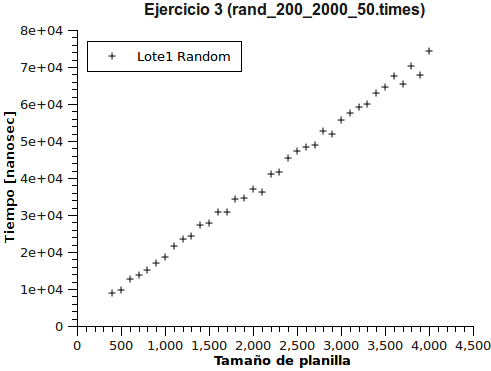
\includegraphics[scale=0.8]{Graph1.png}
\newline
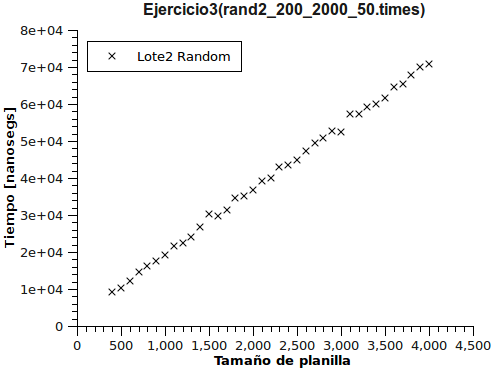
\includegraphics[scale=0.8]{Graph2.png}
\newline
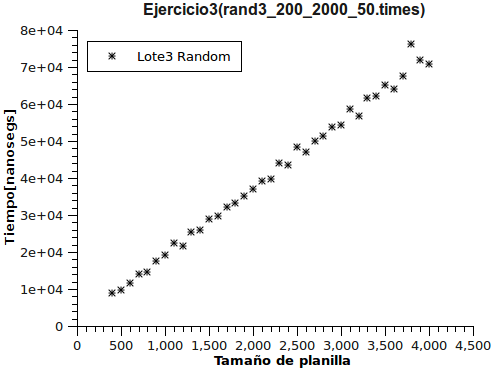
\includegraphics[scale=0.8]{Graph3.png}
\newline


Por otro lado se realizó un lote Worst o Peor caso,(véase \texttt{worst\_200\_2000\_50.in}) y se obtuvo el siguiente gráfico de la tabla de tiempos .

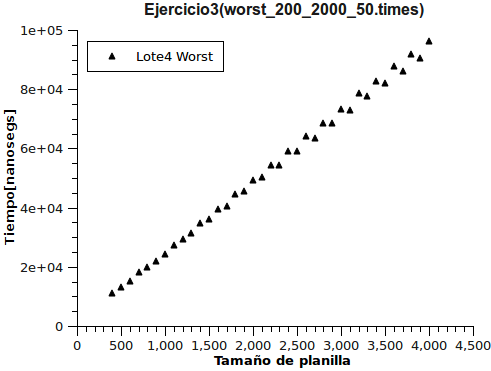
\includegraphics[scale=0.8]{Graph4.png}





\subsection{Conclusiones}

Como era de esperar, el gráfico nos describe una función aproximadamente lineal, observamos que en el que consideramos el peor caso, la pendiente de la 'cuasi recta' es mas pronunciada que en los casos randoms o casos promedio,se puede observar que alcanza valores del orden de $10^{5}$ para planillas de 4000 datos, contra los de orden de $10^{4}$ de los lotes randoms para el mismo tamaño de datos. 
\newline
Sin embargo a los efectos del cálculo de la complejidad, ésto no hace diferencia, ya que la diferencia está dada por una constante multiplicativa .



